\documentclass[conference]{IEEEtran}
\usepackage{cite}
\usepackage{amsmath,amssymb}
\usepackage{graphicx}
\usepackage{textcomp}
\usepackage{xcolor}
\usepackage{booktabs}
\usepackage{multirow}
\usepackage{url}
\usepackage{hyperref}
\usepackage{balance}

\begin{document}

\title{From Passing Tests to Finding Failures: Teaching Exploratory and Robustness-Oriented Testing with Fuzzing}

\author{
\IEEEauthorblockN{
Author One\IEEEauthorrefmark{1}\IEEEauthorrefmark{2},
Author Two\IEEEauthorrefmark{1},
Author Three\IEEEauthorrefmark{1},
Author Four\IEEEauthorrefmark{1}\IEEEauthorrefmark{2}
}
\IEEEauthorblockA{\IEEEauthorrefmark{1}Affiliation One, City, Country}
\IEEEauthorblockA{\IEEEauthorrefmark{2}Affiliation Two, Institution, City, Country}
\{email1, email2, email3\}@domain.com, email4@domain.com
}

\maketitle

\begin{abstract}
Teaching software testing has a persistent blind spot: most curricula train students to confirm that programs work, not to discover how they break.
This paper describes a structured classroom workshop built around grammar-based fuzz testing with \emph{Fandango}, designed to push master's students toward exploratory and robustness-oriented testing thinking.
The workshop unfolds in four phases---conceptual introduction, live crash demonstration, guided hands-on replication, and an open-ended extension where students introduce their own bugs or build new programs to fuzz.
Twenty-two students took part; pre/post self-assessment questionnaires were collected for 20 matched pairs, alongside post-session perception data.
The results are striking in their magnitude: grammar-based fuzzing familiarity improved by $+2.05$ points ($p < 0.001$, $r = 0.877$) and understanding of the random-vs.-grammar distinction by $+2.10$ ($p < 0.001$, $r = 0.877$).
Students found the tool usable (3.90/5) and the session engaging (3.87/5).
Several also spontaneously connected the crashes they observed to potential security vulnerabilities---a finding we did not anticipate.
While the study is limited to a single cohort and a short session, it suggests that grammar-based fuzzing provides a structured, replicable intervention for introducing exploratory and robustness-oriented testing thinking, with empirical evidence of gains in self-assessed familiarity and clear identification of barriers to classroom adoption.
\end{abstract}

\begin{IEEEkeywords}
Fuzz Testing, Software Testing Education, Exploratory Testing, Grammar-Based Fuzzing, Security-Aware Testing, Active Learning
\end{IEEEkeywords}

% ===========================================================================
\section{Introduction}
\label{sec:intro}
% ===========================================================================

A persistent problem in software testing education is that students learn to prove programs right, not to find where they go wrong.
Test cases confirm expected outputs for known inputs---a reasonable starting point, but one that trains a fundamentally optimistic mindset.
The failures that matter most in practice come from inputs nobody anticipated: edge cases, malformed data, adversarial inputs, boundary conditions that expose hidden assumptions.

Consider a developer who writes a command-line calculator and verifies it handles \texttt{ADD 2 3} and \texttt{MUL 4 5}.
All tests pass.
But what happens when someone types \texttt{DIV 7 0}?
Or \texttt{ADD 999999 999999}?
Or simply hits enter without typing anything?
Traditional testing does not look for these failures because it tests what the developer \emph{expects}, not what the program \emph{cannot handle}.

Fuzz testing takes the opposite approach~\cite{miller1990empirical}: it generates unexpected, malformed, or boundary inputs automatically, systematically probing a program's input space.
Grammar-based fuzzing does this with structure---inputs are generated from formal grammar specifications, which keeps them syntactically meaningful and makes the connection between input format and program behavior visible to learners~\cite{aschermann2019nautilus, zeller2019fuzzing}.

Despite widespread industrial use~\cite{manes2019art}, fuzzing rarely appears in software engineering curricula.
The barriers are both practical---perceived complexity, absence of classroom-friendly tooling---and pedagogical: there are few frameworks that connect fuzzing to broader testing goals in a way that makes sense for general courses.

This paper reports a structured classroom workshop using \emph{Fandango}~\cite{fandango2025}, an open-source Python grammar-based fuzzer, designed not as a tool demonstration but as a \emph{mindset intervention}.
The goal was to shift students from asking ``does this produce the right output?'' to asking ``what inputs could break this?''

Three research questions guided the study:
\begin{description}
    \item[RQ1] To what extent does the workshop improve students' self-assessed knowledge and confidence in grammar-based fuzzing and robustness-oriented testing?
    \item[RQ2] How do students perceive the workshop in terms of perceived learning, engagement, usability, and cognitive load?
    \item[RQ3] What conceptual and practical difficulties do students encounter, and what do they reveal about the challenges of introducing fuzzing in educational contexts?
\end{description}

The paper makes three contributions.
First, a four-phase pedagogical design---observe, replicate, break---that progresses from passive observation to active adversarial reasoning and can be replicated in other institutional settings.
Second, empirical evidence of significant self-reported learning gains ($p < 0.001$, large effect sizes $r \geq 0.877$) in grammar-based fuzzing familiarity and related concepts.
Third, a characterization of the practical and conceptual barriers that shape adoption of fuzzing in classroom settings, with implications for how these might be addressed.

% ===========================================================================
\section{Background and Related Work}
\label{sec:background}
% ===========================================================================

\subsection{Software Testing Education and the Testing Mindset}

Software testing occupies an awkward place in most programming curricula.
Students often perceive it as tedious, and the research reflects this: a systematic literature mapping by Garousi et al.~\cite{garousi2020testing} covering more than 200 empirical studies found that instructional effort concentrates heavily on correctness-oriented techniques---unit testing, coverage criteria, test case design---while approaches that target robustness, failure-seeking, or adversarial thinking remain underexplored.
Ammann and Offutt~\cite{ammann2016introduction} make a related observation: students trained on example-based testing develop competent verification skills but may not develop the adversarial intuition needed when the failures that matter are the ones nobody thought to test for.
Novices in particular tend to underestimate the failure space, especially for boundary and malformed inputs~\cite{mccauley2008debugging}.
Robustness-oriented techniques like fuzzing are not just absent from curricula---their absence leaves a genuine gap in how students learn to think about programs.

\subsection{Exploratory and Robustness-Oriented Testing}

Exploratory testing~\cite{whittaker2009exploratory} reframes the activity: rather than confirming that a program does what it should, a tester actively hunts for where it breaks.
Robustness testing narrows this to a specific target---program behavior under abnormal or boundary conditions~\cite{manes2019art}.
Fuzzing operationalizes both at once, exploring the input space automatically and targeting robustness by design, generating the kinds of inputs that human testers rarely think to try.

\subsection{Fuzz Testing: Concepts and Educational Potential}

Fuzzing dates to Miller et al.'s foundational study~\cite{miller1990empirical} and has since become a standard industrial technique~\cite{klees2018evaluating}.
Modern fuzzers like AFL~\cite{afl2021} and LibFuzzer run at scale in industrial codebases.
Grammar-based fuzzing~\cite{aschermann2019nautilus, zeller2019fuzzing} extends the basic idea by generating inputs from formal grammar specifications, producing syntactically structured test cases that make the relationship between input format and program behavior explicit and human-readable.
That transparency is precisely what makes grammar-based fuzzing well-suited for educational settings---students can read, modify, and reason about what the fuzzer produces.

Fuzzing nonetheless remains largely absent from software engineering courses, and when it does appear, it tends to be framed as a security technique rather than a general testing strategy~\cite{klees2018evaluating}.
That framing limits its reach to security-focused courses, even though the underlying skills---systematically exploring how programs fail---are valuable in any engineering context.

\subsection{Hands-on and Experiential Learning in Security and Software Engineering Education}

Learning in software engineering does not happen through passive exposure to concepts; it happens when students grapple with real problems and get immediate feedback on what they try~\cite{kolb1984experiential}.
Kolb's experiential learning model---concrete experience, reflective observation, active experimentation~\cite{kolb1984experiential}---maps directly onto the workshop structure described here.
Problem-based learning~\cite{hmelo2004problem} and inquiry-based instruction~\cite{prince2004active} reinforce the same point: give students a genuine problem without a predetermined answer and let them work through it.

Hands-on laboratory exercises have proven effective in security and software engineering education, where direct exposure to realistic failure modes and adversarial conditions builds both technical skill and security-aware reasoning~\cite{du2011seed}.
The emergent finding in this study---that students spontaneously drew connections between observed crashes and potential vulnerabilities---fits squarely within that pattern.

Prior work has examined software testing education, active learning, and fuzzing as a professional technique extensively. What is missing is an account of how grammar-based fuzzing can be operationalized as a short, scaffolded, and empirically evaluated classroom activity accessible to general software engineering students. This paper is an attempt to address that gap, through a four-phase workshop that treats grammar-based fuzzing as a vehicle for failure-seeking thinking rather than a security specialization.

% ===========================================================================
\section{Methodology}
\label{sec:methodology}
% ===========================================================================

\subsection{Participants and Context}

Twenty-two master's students enrolled in a software engineering course at the Universidade da Beira Interior, Portugal took part in the study.
Most (21 of 22) came from Computer Science or Software Engineering programs and had intermediate programming experience.
Very few had encountered fuzz testing before.
Participation in the evaluation component was voluntary, anonymous, and conducted under informed consent.

\subsection{Workshop Design}

The workshop ran for approximately 100~minutes and followed the four-phase structure shown in Fig.~\ref{fig:workflow}.

\begin{figure}[t]
\centering
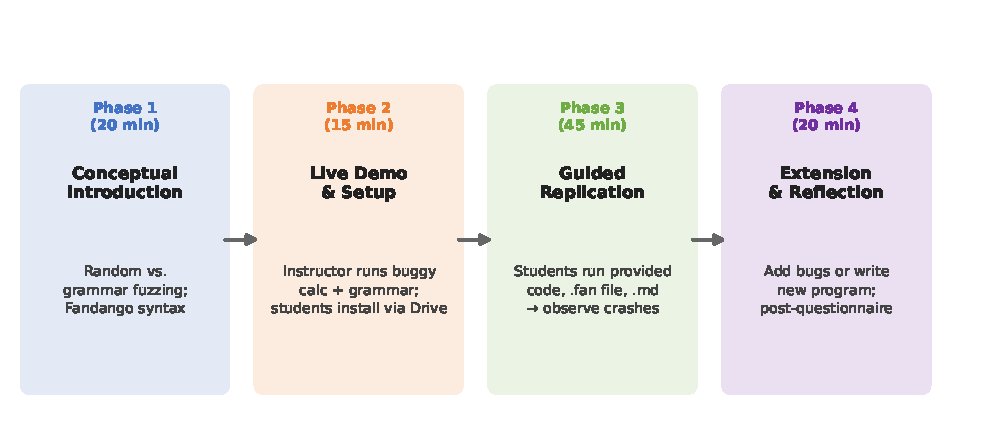
\includegraphics[width=\columnwidth]{figures/fig_fandango_workflow.pdf}
\caption{Workshop workflow: four progressive phases from conceptual introduction to open-ended extension.}
\label{fig:workflow}
\end{figure}

\subsubsection{Phase 1 --- Conceptual Introduction (20~min)}
The session opened with a critique of example-based testing: why does confirming that \texttt{ADD 2 3} returns 5 not tell us whether \texttt{DIV 7 0} crashes the program?
The instructor introduced fuzz testing as a response to this limitation, explained the distinction between random and grammar-based fuzzing, and walked through the Fandango grammar syntax with a live example.

\subsubsection{Phase 2 --- Live Demonstration (15~min)}
The instructor ran a live fuzzing session against a deliberately buggy Python calculator program, using a pre-written Fandango grammar file (\texttt{.fan}).
Students watched crashes appear in real time as the fuzzer generated inputs like \texttt{DIV 7 0} and malformed expressions.
The instructor then analyzed one crash trace with the class---tracing the fault, identifying its root cause, and sketching what a defensive fix would look like.

\subsubsection{Phase 3 --- Guided Replication (45~min)}
Students received all materials via Google Drive---the buggy calculator, the grammar file, and a step-by-step Markdown guide (\texttt{.md}) for setting up a Python virtual environment and running the fuzzer.
They installed Fandango, ran the grammar, and reproduced the crashes the instructor had demonstrated.
Once they had the basic pipeline working, students were guided to modify the grammar to generate new input classes (e.g., negative numbers, very large values, empty strings) and observe how each change affected which crashes were found.

\subsubsection{Phase 4 --- Open-Ended Extension (20~min)}
In the final phase, students chose between two activities: introducing deliberate bugs into the calculator and checking whether the fuzzer could detect them, or writing a new Python program from scratch and building a grammar for it.
The aim was to reason from both sides simultaneously---as a developer who knows where the bugs are and as a tester who has to find them.
A short group reflection and the post-session questionnaire closed the session.

\subsection{Data Collection}

\subsubsection{Pre-Activity Questionnaire}
Background questions on academic field, programming experience, and prior tool use; seven Likert self-assessment items (5-point scale) covering: fuzz testing familiarity, grammar-based fuzzing familiarity, CLI confidence, edge-case understanding, automated test generation understanding, crash interpretation confidence, and understanding of the random-vs.-grammar distinction; one MCQ on grammar-based fuzzing definition.

\subsubsection{Post-Activity Questionnaire}
The same seven Likert items and MCQ, plus post-only constructs: perceived learning (5~items), engagement (3~items), usability (2~items), cognitive load (3~items), and four open-ended questions.

\subsubsection{Anonymous Matching}
Students generated a personal code (last two digits of phone number + birth month + first letter of first name) used across both questionnaires.
Of 22 participants, 20 provided matched pre/post responses; one completed only the pre-session questionnaire.
All paired analyses use $N = 20$.

\subsection{Data Analysis}

Pre/post Likert differences were tested using the Wilcoxon signed-rank test; effect size was computed as $r = |Z|/\sqrt{N}$.
Construct means were computed for post-session perception items.
Open-ended responses were analyzed using lightweight thematic coding.

% ===========================================================================
\section{Results}
\label{sec:results}
% ===========================================================================

\subsection{RQ1: Grammar-Based Fuzzing Knowledge and Robustness-Oriented Confidence}

Table~\ref{tab:likert} reports pre/post self-assessment for all seven items ($N = 20$).
Fig.~\ref{fig:prepost} shows the shifts visually.

\begin{table}[htbp]
\caption{Pre/Post Self-Assessment ($N = 20$)}
\label{tab:likert}
\centering
\small
\begin{tabular}{lccccc}
\toprule
Item & Pre & Post & $\Delta$ & $p$ & $r$ \\
\midrule
Fuzz familiarity         & 1.80 & 3.55 & +1.75 & $<$\,.001 & .855 \\
Grammar-fuzz famil.      & 1.60 & 3.65 & +2.05 & $<$\,.001 & .877 \\
CLI confidence           & 2.90 & 3.50 & +0.60 & .017 & .567 \\
Edge-case underst.       & 3.60 & 3.85 & +0.25 & .322 & .285 \\
Auto-test generation     & 3.70 & 4.10 & +0.40 & .091 & .422 \\
Crash interpretation     & 3.00 & 3.45 & +0.45 & .033 & .513 \\
Random vs.\ grammar      & 1.65 & 3.75 & +2.10 & $<$\,.001 & .877 \\
\bottomrule
\end{tabular}
\end{table}

\begin{figure}[htbp]
\centering
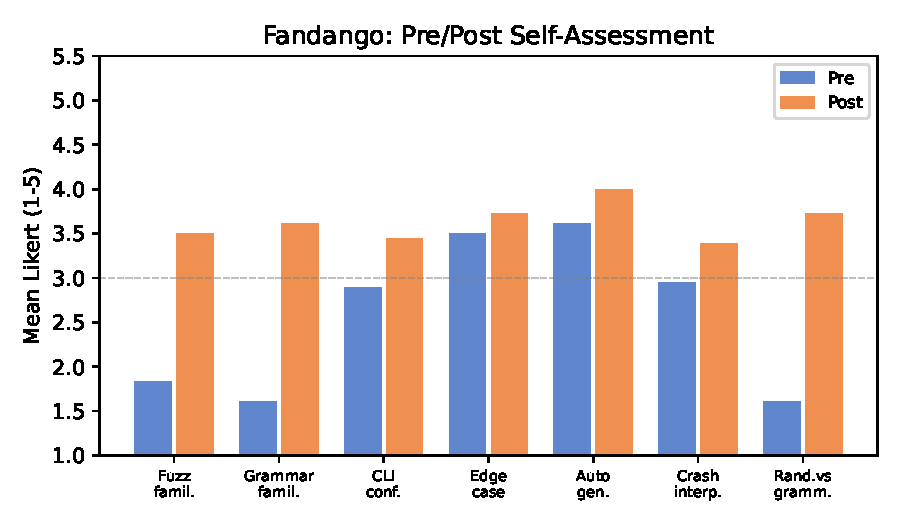
\includegraphics[width=\columnwidth]{figures/fig_fandango_prepost.pdf}
\caption{Pre/post self-assessment across seven Likert items. Largest gains on items directly addressed by the workshop.}
\label{fig:prepost}
\end{figure}

The gains on grammar-based fuzzing items were large by any measure.
Familiarity with grammar-based fuzzing rose by $+2.05$ points ($p < 0.001$, $r = 0.877$, large effect), understanding of the random-vs.-grammar distinction by $+2.10$ ($p < 0.001$, $r = 0.877$), and general fuzz testing familiarity by $+1.75$ ($p < 0.001$, $r = 0.855$).
The effect sizes are partly explained by the pre-session baseline: means around 1.6 on a 5-point scale indicate that students arrived with almost no prior exposure to fuzzing.

Robustness-oriented competencies told a more mixed story.
Crash interpretation improved significantly ($+0.45$, $p = 0.033$, $r = 0.513$) and CLI confidence showed a meaningful gain ($+0.60$, $p = 0.017$, $r = 0.567$).
Edge-case understanding and automated test generation moved in the right direction but did not reach significance ($p > 0.05$)---a pattern consistent with these being broader robustness competencies that take more than a single session to develop.

\subsection{RQ2: Student Perception}

Table~\ref{tab:perception} summarizes post-session perception ($N = 20$), with Fig.~\ref{fig:perception} providing a visual overview.

\begin{table}[htbp]
\caption{Post-Session Perception ($N = 20$)}
\label{tab:perception}
\centering
\small
\begin{tabular}{lcc}
\toprule
Construct (items) & Mean & \% Agree \\
\midrule
Perceived Learning (5) & 3.73 & 60\% \\
Engagement (3)         & 3.87 & 62\% \\
Usability (2)          & 3.90 & 68\% \\
Cognitive Load (3)     & 3.32 & --- \\
\bottomrule
\end{tabular}
\end{table}

\begin{figure}[htbp]
\centering
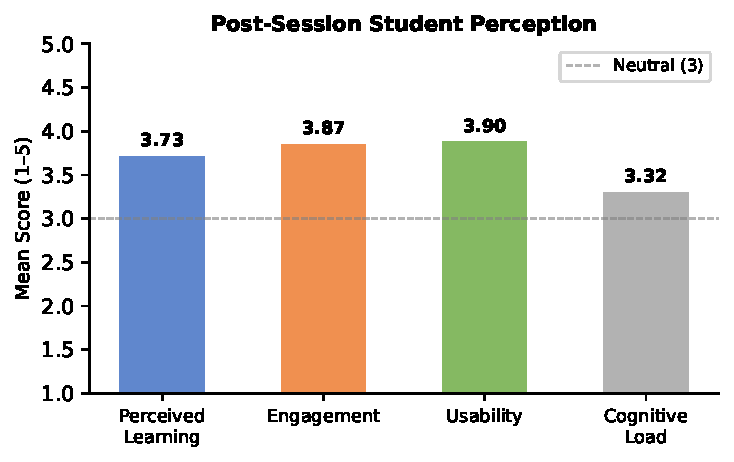
\includegraphics[width=\columnwidth]{figures/fig_fandango_perception.pdf}
\caption{Post-session perception: mean scores across four constructs. Dashed line indicates neutral (3).}
\label{fig:perception}
\end{figure}

Students' reactions to the session were broadly positive.
Perceived learning landed at a moderate 3.73/5 (60\% agree)---lower than the other constructs, which likely reflects the conceptual novelty of fuzzing rather than dissatisfaction with the workshop itself.
Engagement reached 3.87/5 (62\% agree).
Usability came in highest at 3.90/5, suggesting that once students got Fandango installed and running, the tool itself was not an obstacle.
Cognitive load was moderate (3.32/5), reflecting the genuine complexity of learning a new tool and a new mode of thinking simultaneously.
Because the cognitive-load items showed lower internal consistency, this construct is interpreted descriptively rather than as a validated scale score.

\subsection{RQ3: Student Difficulties and What They Reveal}

Thematic analysis of open-ended responses turned up two recurring categories of difficulty alongside two themes that were unexpectedly positive.

\textbf{Practical difficulties.}
Installation dominated the complaints.
Students struggled particularly on Windows (\emph{``problems installing Fandango,''} \emph{``version of Python,''} \emph{``pre requirements to make the activity run''}), with environment setup consuming time that could have gone to the hands-on work and, in some cases, preventing students from getting there at all.
This is a familiar pattern with CLI-based educational tools: environment configuration is genuinely hard in a heterogeneous classroom, and it showed up clearly here.

\textbf{Conceptual difficulties.}
The other consistent obstacle was the grammar syntax itself.
Students found the formal specification unfamiliar---one described the challenge as \emph{``Maybe, at the beginning, to understand the difference between random fuzzing and grammar-based fuzzing''}.
The cognitive shift required to think in formal grammars rather than in procedural assertions is real, and it represents the kind of threshold concept that does not dissolve on its own without dedicated scaffolding.

\textbf{Emergent themes.}
Two things emerged that we had not specifically set out to measure.
Several students spontaneously connected the crashes they observed to security vulnerabilities (\emph{``Analysing software crashes,''} \emph{``Crash demonstration''}), an association the workshop never made explicit.
Students also requested more time with the hands-on work---\emph{``Maybe try to add an extra exercise that try to simulate a more realistic and complex working scenario,''} \emph{``More pratical~[sic] in more hours''}---which suggests the open-ended extension phase was seen as the most valuable part of the session, not merely an afterthought.

% ===========================================================================
\section{Discussion}
\label{sec:discussion}
% ===========================================================================

\subsection{The Pedagogical Progression: Observe, Reproduce, Break}

The three-phase structure---live demonstration, guided replication, open-ended extension---worked as a scaffolding sequence, each step shifting cognitive demand a little further from observation toward active construction.

The live demonstration (Phase 2) did something a lecture slide cannot: it showed students a program they already understood crashing in front of them, for reasons they had not anticipated.
Seeing \texttt{DIV 7 0} trigger an unhandled exception is a different experience from reading about it.
Students did not just hear that programs can break in unexpected ways; they watched it happen.

Phase 3 moved responsibility to the students.
Having all materials pre-prepared meant they could focus on reproducing the experience and then experimenting with the grammar, rather than spending the session debugging their environment.
The step-by-step guide served as scaffolding that students could step off of once the pipeline was running.

Phase 4 was where the more interesting learning happened, or at least where students report it did.
Open-ended responses suggest this phase was particularly valuable, though we should be honest about the limits of that observation: no systematic log data was collected to verify how many students completed it or what they found.
The value of the phase lies in the perspective shift it demands---understanding not just that programs fail, but why they fail and how to construct inputs that expose specific failure modes.

\subsection{Fuzzing as a Security Awareness Gateway}

We did not design the workshop around security.
Yet several students, without any prompting, connected the crashes they observed to potential vulnerabilities.
This is worth noting carefully: it is an emergent finding from open-ended responses, not something we measured, and stronger claims would require a dedicated study.
But it is consistent with what the hands-on security education literature would predict---when students interact directly with program failures, they begin to think about who might cause those failures intentionally.

\subsection{Practical and Conceptual Barriers: Implications for Curriculum Design}

The two categories of difficulty identified in RQ3 call for different responses.

Installation friction is a practical problem with practical solutions.
It consumes class time and excludes students who cannot get the environment working.
At the same time, dependency management and platform-specific configuration are authentic features of real software development; exposure to them---with support available---is not without educational value.
A hybrid approach seems sensible: provide a pre-configured cloud environment as a fallback while still walking students through the installation, preserving the authentic experience for those who can complete it.

The grammar specification barrier is harder to address.
Students accustomed to procedural testing---write an assertion, check an output---have to shift to a different mode of thinking when they encounter formal grammars.
That shift is not obvious, and it does not happen on its own.
Dedicating more explicit instructional time to it, and connecting it to formal notations students have already encountered (regular expressions, context-free grammars from a compilers course), would likely lower the threshold.

\subsection{Limitations of a Single Session}

Non-significant results for edge-case understanding ($p = 0.322$) and automated test generation ($p = 0.091$) are not surprising.
These are broad competencies that a 100-minute workshop was never realistically going to transform.
What a single session can do is introduce the vocabulary, motivate the mindset, and demonstrate the technique convincingly enough that students leave curious rather than confused.
Sustained curriculum integration is what it takes to develop deeper skill.
Future workshops should build on this foundation with more complex grammars, multi-session activities, and integration with complementary techniques such as property-based testing and mutation testing.

% ===========================================================================
\section{Threats to Validity}
\label{sec:threats}
% ===========================================================================

\textbf{Internal validity.}
Without a control group, we cannot rule out alternative explanations for the observed gains.
Reuse of identical MCQ items across pre and post may also introduce a testing effect.

\textbf{Construct validity.}
The Likert items measure self-reported familiarity and confidence, not actual skill acquisition.
They were designed for this study and carry no external validation.

\textbf{External validity.}
A single cohort of 22 students at one Portuguese university is a narrow sample.
How well these results generalize to students with different backgrounds, different target programs, or different Fandango versions remains an open question.

\textbf{Reliability.}
Internal consistency was good for perceived learning ($\alpha = 0.879$), engagement ($\alpha = 0.858$), and usability ($\alpha = 0.812$).
Cognitive load items showed lower consistency due to mixed item valence and are interpreted descriptively throughout.

% ===========================================================================
\section{Conclusion}
\label{sec:conclusion}
% ===========================================================================

Grammar-based fuzzing is an unusual teaching tool: it generates failures automatically, makes the relationship between input structure and program behavior visible, and produces results immediately.
This paper described a workshop built around those properties, designed to shift students from correctness-focused testing toward a failure-seeking mindset.

The empirical picture is encouraging.
Familiarity with grammar-based fuzzing rose by $+2.05$ ($p < 0.001$, $r = 0.877$) and understanding of the random-vs.-grammar distinction by $+2.10$ ($p < 0.001$, $r = 0.877$).
Students found the session engaging and the tool usable, and several made an unprompted connection between the crashes they observed and potential security vulnerabilities---a finding that warrants further investigation.

Overall, the findings suggest that grammar-based fuzzing can serve as a practical and engaging classroom pathway into exploratory and robustness-oriented testing.
However, broader competence development requires sustained curricular integration beyond a single workshop.
Future work should investigate what a multi-session version of this workshop looks like, how the learning holds up over time, and how grammar-based fuzzing integrates with complementary techniques like mutation testing and property-based testing.

\section*{Data Availability}
The replication package---including questionnaire data, analysis scripts, and workshop materials---is publicly available at: \url{https://github.com/aazaadef/Fandango-Workshop}

\section*{Acknowledgment}
This work was supported by FCT -- Funda\c{c}\~{a}o para a Ci\^{e}ncia e Tecnologia, I.P.\ by project reference UIDB/50008/2020 (DOI: \url{https://doi.org/10.54499/UIDB/50008/2020}) and by the doctoral grant PRT/BD/155023/2023.
The authors would also like to acknowledge the Promptme4Better project, funded by the European Union Erasmus+ Program and the Portugal National Agency under grant agreement number 2025-1-PT01-KA220-HED-000363565, and all partners involved in the project.
The authors used generative AI tools solely to support English language polishing and readability improvements.
All technical content, interpretations, and conclusions were created and verified by the authors, who take full responsibility for the final manuscript.

\balance
\bibliographystyle{IEEEtran}
\begin{thebibliography}{99}
\bibitem{fandango2025} ``Fandango: Grammar-Based Fuzzing Tool,'' 2025. Available: https://github.com/fandango-fuzzer/fandango
\bibitem{miller1990empirical} B.~P.~Miller, L.~Fredriksen, and B.~So, ``An Empirical Study of the Reliability of UNIX Utilities,'' \emph{Commun.\ ACM}, vol.~33, no.~12, pp.~32--44, 1990.
\bibitem{manes2019art} V.~J.~M.~Man\`{e}s et~al., ``The Art, Science, and Engineering of Fuzzing: A Survey,'' \emph{IEEE Trans.\ Softw.\ Eng.}, vol.~47, no.~11, pp.~2312--2331, 2021.
\bibitem{klees2018evaluating} G.~Klees et~al., ``Evaluating Fuzz Testing,'' in \emph{Proc.\ CCS '18}, ACM, 2018, pp.~2123--2138.
\bibitem{aschermann2019nautilus} C.~Aschermann et~al., ``NAUTILUS: Fishing for Deep Bugs with Grammars,'' in \emph{Proc.\ NDSS '19}, 2019.
\bibitem{zeller2019fuzzing} A.~Zeller, R.~Gopinath, M.~B\"{o}hme, G.~Fraser, and C.~Holler, ``The Fuzzing Book,'' 2019. Available: https://www.fuzzingbook.org/
\bibitem{afl2021} M.~Zalewski, ``American Fuzzy Lop (AFL),'' 2021. Available: https://lcamtuf.coredump.cx/afl/
\bibitem{whittaker2009exploratory} J.~A.~Whittaker, \emph{Exploratory Software Testing}. Addison-Wesley, 2009.
\bibitem{ammann2016introduction} P.~Ammann and J.~Offutt, \emph{Introduction to Software Testing}, 2nd~ed. Cambridge University Press, 2016.
\bibitem{garousi2020testing} V.~Garousi, A.~Rainer, P.~Lauv\aa{}s~Jr., and A.~Arcuri, ``Software-testing education: A systematic literature mapping,'' \emph{J.\ Syst.\ Softw.}, vol.~165, 2020.
\bibitem{mccauley2008debugging} R.~McCauley et~al., ``Debugging: a review of the literature from an educational perspective,'' \emph{Comput.\ Sci.\ Educ.}, vol.~18, no.~2, pp.~67--92, 2008.
\bibitem{kolb1984experiential} D.~A.~Kolb, \emph{Experiential Learning: Experience as the Source of Learning and Development}. Prentice-Hall, 1984.
\bibitem{hmelo2004problem} C.~E.~Hmelo-Silver, ``Problem-Based Learning: What and How Do Students Learn?'' \emph{Educ.\ Psychol.\ Rev.}, vol.~16, no.~3, pp.~235--266, 2004.
\bibitem{prince2004active} M.~Prince, ``Does Active Learning Work? A Review of the Research,'' \emph{J.\ Eng.\ Educ.}, vol.~93, no.~3, pp.~223--231, 2004.
\bibitem{du2011seed} W.~Du, ``SEED: Hands-on Lab Exercises for Computer Security Education,'' \emph{IEEE Secur.\ Priv.}, vol.~9, no.~5, pp.~70--73, 2011.
\end{thebibliography}

\end{document}
